
\chapter{AI-Driven Optimization and Secure Autonomy in UAV Systems}


%%%%%%%%%%%%%%%%%%%%%%%%%%%%%%%%%%%%%%%%%%%%%%%%%%%%%%%%%%%%%%%%%%%%%%
%%%%%%%%%%%%%%%%%%%%%%%%%%%%%%%%%%%%%%%%%%%%%%%%%%%%%%%%%%%%%%%%%%%%%%
%%%%%%%%%%%%%%%%%%%%%%%%%%%%%%%%%%%%%%%%%%%%%%%%%%%%%%%%%%%%%%%%%%%%%%



\section*{Introduction}


Unmanned Aerial Vehicles (UAVs) have become indispensable in fields such as agriculture, surveillance, and disaster response, thanks to their agility and advanced sensing capabilities. A key driver of their success is the integration of Artificial Intelligence (AI) and optimization techniques, which improve trajectory planning, mission efficiency, and real-time decision-making. This chapter examines how machine learning including supervised, unsupervised, and reinforcement learning enhances UAV operations, from energy-efficient navigation to dynamic feature extraction. It also addresses critical security risks in UAV networks, such as jamming, spoofing, and malicious attacks, while discussing countermeasures. By reviewing advancements in AI-driven optimization and cybersecurity, this chapter establishes a foundation for understanding the current state of UAV technology and its future directions.


%%%%%%%%%%%%%%%%%%%%%%%%%%%%%%%%%%%%%%%%%%%%%%%%%%%%%%%%%%%%%%%%%%%%%%
%%%%%%%%%%%%%%%%%%%%%%%%%%%%%%%%%%%%%%%%%%%%%%%%%%%%%%%%%%%%%%%%%%%%%%
%%%%%%%%%%%%%%%%%%%%%%%%%%%%%%%%%%%%%%%%%%%%%%%%%%%%%%%%%%%%%%%%%%%%%%



\section{Machine learning optimization for UAVs}



%%%%%%%%%%%%%%%%%%%%%%%%%%%%%%%%%%%%%%%%%%%%%%%%%%%%%%%%%%%%%%%%%%%%%%


%AI

\subsection{ML for UAV trajectory planning and mission scheduling}


In recent years, machine learning (ML) has played a significant role in enhancing flight control strategies to improve the overall quality of UAV services. By strategically planning trajectories, UAVs are able to collect data from target nodes while ensuring that the information remains up to date. Supervised learning methods are commonly employed to reduce training errors, which contributes to more efficient trajectory design. In addition, reinforcement learning techniques such as Deep Q-Networks (DQN) and Deep Deterministic Policy Gradient (DDPG) offer strong predictive and classification capabilities, making them suitable for both discrete and continuous action space environments. These reinforcement learning approaches are widely used in UAV trajectory optimization and mission scheduling.


%%%%%%%%%%%%%%%%%%%%%%%%%%%%%%%%%%%%%%%%%%%%%%%%%%%%%%%%%%%%%%%%%%%%%%


\subsubsection{Supervised Learning-based UAV Communications}



The prediction of UAV flight paths has been explored in the context of communication services within smart cities. In such scenarios, having precise information about the UAV’s position is essential, since it directly affects the beamforming process conducted by the connected base station. A method based on recurrent neural networks (RNNs) for predicting the angle of arrival, supported by a set of data preprocessing steps, has shown promising results. Simulation outcomes demonstrate that this method can successfully learn and adapt angle data, making it suitable for UAVs operating at high speeds.

A related application is presented in~\cite{annepu2020uav}, where a UAV functions as a dynamic aerial anchor to assist in locating ground-based sensors. It estimates the sensor positions by measuring the received signal strength (RSS) from them. Compared to traditional fixed ground anchors, the use of UAVs enhances localization accuracy due to the dominance of line-of-sight (LOS) paths. As illustrated in Fig.~\ref{fig:mlp-uav-localization}, a multilayer perceptron (MLP) model is constructed to predict sensor locations using RSS values as input features. The MLP is trained using the backpropagation algorithm, with training samples consisting of randomly distributed node positions within a sensor field. Thanks to its nonlinear activation functions, the MLP can effectively model the log-normal shadow fading, achieving up to 35\% better localization precision than non-ML-based techniques. This approach is further improved through the use of radial basis function models, as proposed in~\cite{annepu2021radial}.




%%%%%%%%%%%%%%%%%%%%%%%%%%%%%%%%%%%%%%%%%%%%%%%%%%%%%%%%%%%%%%%%%%%%%%



\subsubsection{Unsupervised Learning for Trajectory Planning and
 Communications}


Unsupervised learning techniques, such as autoencoders, GANs, and GMMs, have been applied to UAV trajectory planning and communications. Autoencoders generate waypoints through a three-step process: extracting potential waypoints from historical trajectories, creating trajectory-based images, and identifying waypoints via repeating pixel patterns. This approach reduces waypoints by 84.21\% compared to K-means, enhancing energy efficiency. Autoencoders also predict movement in dynamic environments by reconstructing action-conditioned video frames for trajectory planning. For attitude control, deep autoencoders with multiple hidden layers fuse data from gyroscopes, accelerometers, and magnetometers, outperforming single-layer architectures in attitude estimation through restricted Boltzmann machine-based networks.


\begin{figure}[H]
\centering
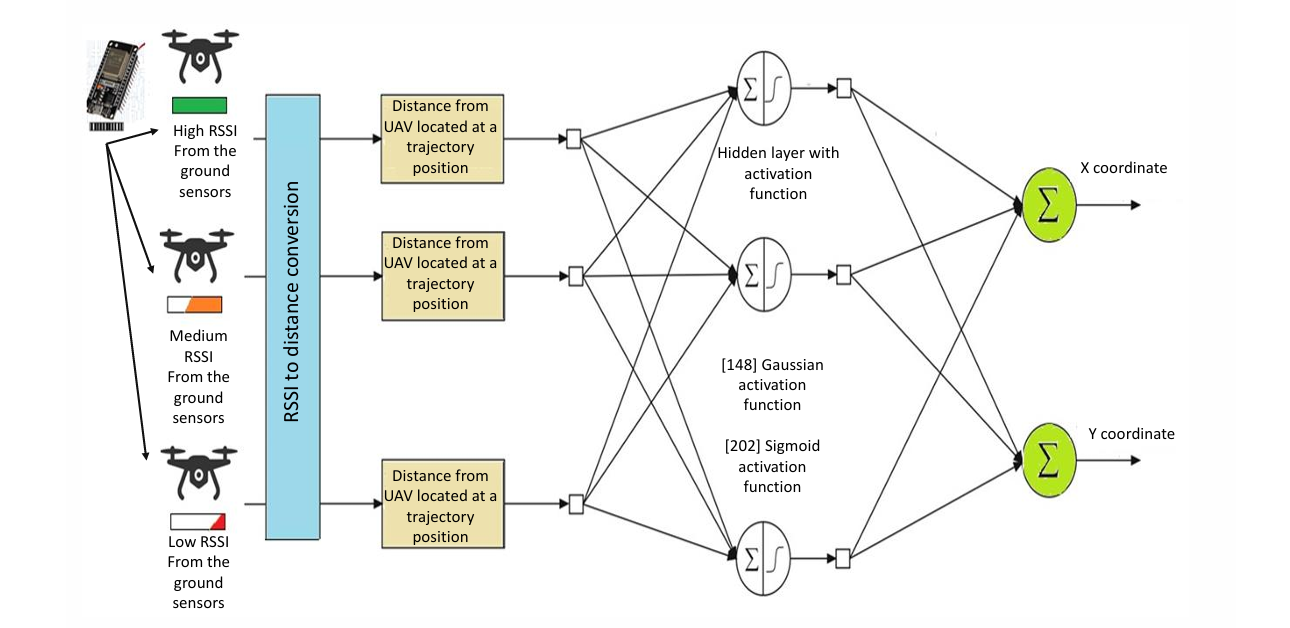
\includegraphics[width=0.7\textwidth]{Figures/Chapter2/Section1/1.png}
\caption{The MLP for UAV-based localization of a WSN node using the Gaussian activation function \cite{annepu2020uav} and the RBF model
 using the Sigmoid activation function \cite{annepu2021radial}}
\label{fig:mlp-uav-localization}
\end{figure}


In UAV-aided image analysis, challenges like camera pose variations, shadows, and illumination changes often stem from noise or acquisition issues. Autoencoders address these by clustering image features based on similarity, with the encoder network learning to distinguish dynamic changes through training and reduces the required number of training images.




%%%%%%%%%%%%%%%%%%%%%%%%%%%%%%%%%%%%%%%%%%%%%%%%%%%%%%%%%%%%%%%%%%%%%%

\subsubsection{ Semi-supervised Learning for UAV Trajectory Opti
mization}



A Generative Adversarial LSTM (GA-LSTM) network can be used to optimize resource allocation in UAV-assisted machine-to-machine wireless communications. This architecture combines the capabilities of Generative Adversarial Networks (GANs) and Long Short-Term Memory (LSTM) networks to jointly optimize transmit power, communication mode, frequency channel selection, and UAV selection and trajectory within a partially observable multi-agent environment. The LSTM component enables the tracking of UAV movements and supports reward evaluation. Numerical evaluations show that this integrated model achieves higher sum rates compared to standalone LSTM or Deep Q-Network (DQN) methods.

In cellular networks that include both UAV-based aerial base stations (BSs) and ground BSs, a Gaussian Mixture Model (GMM) with weighted expectation-maximization can be employed to represent the spatial traffic distribution and guide base station deployment, including UAV positioning. This technique allows for traffic congestion prediction and determines the optimal placement of UAVs to reduce energy costs related to both communication and relocation. Simulation results highlight energy savings of up to 20\% for communication and 80\% for relocation when compared to heuristic approaches.




%%%%%%%%%%%%%%%%%%%%%%%%%%%%%%%%%%%%%%%%%%%%%%%%%%%%%%%%%%%%%%%%%%%%%%

\subsubsection{Reinforcement Learning for Joint Trajectory Plan
ning and Mission Scheduling}


Deep Reinforcement Learning (DRL) techniques offer innovative approaches for planning UAV trajectories in dynamic environments.


\paragraph{Deep Q-Network with Trajectory Discretization}




In UAV-assisted communications, reinforcement learning approaches like Q-learning face challenges with large state/action spaces, prompting the use of Deep Q-Networks (DQNs) which leverage neural networks to handle extended spaces. DQNs have been particularly effective for Age of Information optimization, where they balance energy efficiency with data freshness while using autoencoders with LSTM to manage large state spaces through spatiotemporal feature extraction ~\cite{abedin2020data,ferdowsi2021neural}.


\begin{figure}[H]
\centering
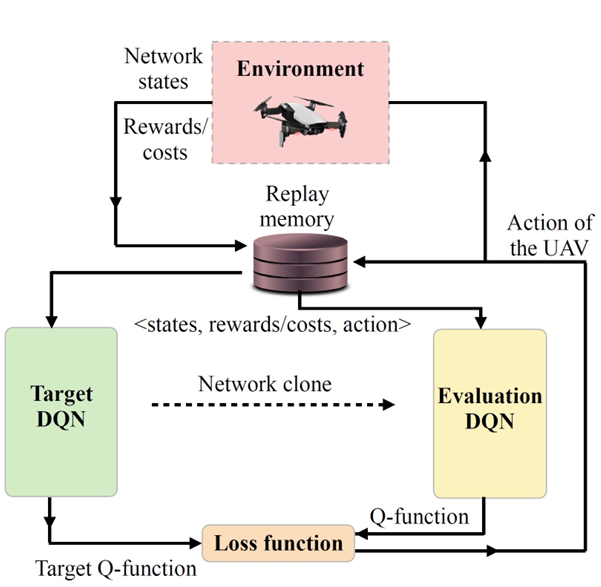
\includegraphics[width=0.7\textwidth]{Figures/Chapter2/Section1/2.png}
\caption{ Schematic overview of a DQN-based framework for UAV trajectory and mission planning. The model is deployed onboard the UAV and trained to generate optimal policies for both path planning and radio resource allocation. \cite{kurunathan2022machine}}
\label{fig:dqn_trajectory_planning}
\end{figure}



For throughput and energy optimization, deep Q-networks (DQNs) are used to jointly optimize UAV trajectories and bandwidth allocation. These methods take into account node states and data volume to enhance overall network performance. Packet loss issues are mitigated by adjusting UAV velocity and scheduling communications based on real-time data, including battery levels, queue statuses, and channel conditions.

In coverage-oriented applications, DQNs are applied to maintain robust network connectivity. They dynamically adapt to changes in topology and optimize UAV paths to balance coverage fairness and energy consumption. Advanced versions such as dueling DQNs are employed for scenarios requiring optimized flight paths for uplink throughput. These approaches also integrate obstacle avoidance and prioritize data with latency sensitivity.

In UAV-assisted Mobile Edge Computing (MEC) systems, double DQNs support effective task offloading decisions. This improves throughput while managing energy limitations and addressing data security challenges like eavesdropping. Wireless power transfer systems benefit from DQN-based optimization techniques as well, especially for planning UAV trajectories and selecting energy-harvesting nodes. These strategies are sometimes enhanced using probabilistic algorithms such as Naive Bayes for estimating node locations.

Although these techniques have broad applicability, their reliance on discrete action spaces poses a limitation. This constraint reduces their suitability for continuous control problems, such as fine-tuned UAV cruise control, highlighting the need for alternative or hybrid approaches in such contexts.




%%%%%%%%%%%%%%%%%%%%%%%%%%%%%%%%%%%%%%%%%%%%%%%%%%%%%%%%%%%5

\paragraph{Online Trajectory Planning With Deep Deterministic
 Policy Gradient}



The Deep Deterministic Policy Gradient (DDPG) algorithm effectively combines value iteration and policy iteration approaches, offering a robust framework for deep reinforcement learning in continuous state and action spaces. Unlike Deep Q-Networks (DQN), which predict Q-values for discrete state-action pairs, DDPG employs a dual-network structure: a critic network that estimates Q-values and an actor network that determines optimal actions. This architecture allows DDPG to manage continuous control problems more efficiently than traditional DQN methods.

\begin{enumerate}

\item \textbf{Cruise Control:} DDPG demonstrates strong capabilities in UAV cruise control by learning optimal headings and velocities to minimize network costs in continuous action spaces. Its experience replay mechanism improves training stability by reusing past learning samples. Applications include autonomous landing on dynamic platforms, air combat maneuvering through precise trajectory control, and urban navigation that integrates obstacle avoidance with energy-efficient route planning.

\item \textbf{Age of Information (AoI):} DDPG is effective in minimizing the Age of Information by adapting to dynamic traffic and environmental conditions. Advanced variants like twin delayed DDPG (TD3) improve energy efficiency while maintaining low AoI in IoT networks. Multi-agent extensions enhance trajectory learning, and policy-based enhancements enable optimization of flight altitude and transmission scheduling.

\item \textbf{UAV-assisted MEC:} In Mobile Edge Computing scenarios, DDPG handles complex action spaces, making it suitable for joint optimization of content caching, delivery, and power control. It plays a key role in vehicular networks, managing spectrum and computing resource allocation and addressing the multifaceted challenges of UAV-assisted MEC environments.

\item \textbf{Other Applications:}
\begin{itemize}
    \item Deep reinforcement learning-based frameworks have achieved improved fairness and energy efficiency in coverage and resource allocation.
    \item Game-theoretic approaches combined with DDPG enable optimal UAV deployment and trajectory planning while ensuring obstacle avoidance.
    \item Hybrid systems integrating DDPG with LSTM networks facilitate dynamic spectrum sharing through intelligent timeslot allocation.
    \item Enhanced Q-network variants have been applied to outage minimization and integrated navigation with radio environment mapping.
\end{itemize}

\end{enumerate}





\begin{figure}[ht]
\centering
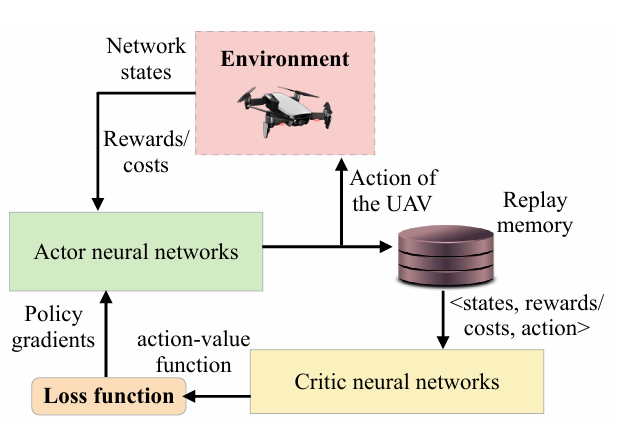
\includegraphics[width=0.7\textwidth]{Figures/Chapter2/Section1/4.png}
\caption{DDPG Architecture Overview with Actor-Critic Networks and Experience Replay for UAV Control \cite{kurunathan2022machine}}
\label{fig:ddpg_uav_control}
\end{figure}


%%%%%%%%%%%%%%%%%%%%%%%%%%%%%%%%%%%%%%%%%%%%%%%%%%%%%%%%%%%

\paragraph{Multi-agent DRL for Multi-UAV Cooperation}

The multi-agent DQN framework has been successfully implemented for cooperative UAV systems, where the network state incorporates ground nodes' battery levels, data queue statuses, and all UAV waypoints~\cite{dqn_multi_115}. This approach enables intelligent scheduling of ground node transmissions while dynamically adapting to changing data and energy arrival patterns.

Building upon this foundation, researchers have enhanced the multi-agent DQN framework to incorporate velocity adjustment capabilities at waypoints, while maintaining optimal ground node selection for data transmission. This extension provides more refined control over UAV movements during mission execution.

For cellular network applications, multi-agent DQN can effectively address the complex joint optimization of UAV trajectories and communication scheduling. The solution coordinates data transmissions from cellular tower ground nodes based on relative positions between UAVs and ground stations.

In energy conservation scenarios, a non-cooperative game formulation with periodic UAV beaconing establishes optimal beaconing equilibrium durations without requiring knowledge of other UAVs' transmission schedules.

Security applications have leveraged multi-agent DDPG approaches, where UAV jammers are coordinated to enhance secure channel capacity. The framework simultaneously optimizes jammer trajectories, jamming power levels, and legitimate UAV transmission power.

For MEC systems, a multi-agent DDPG model improves resource allocation fairness while optimizing UAV trajectories and computation offloading decisions to boost MEC device energy efficiency.

Further advancing MEC applications, a comprehensive multi-agent DDPG framework for vehicular networks treats the MEC server as an intelligent agent coordinating UAV and ground vehicle scheduling, along with computational resource allocation. Integration with federated learning significantly improves task offloading performance from vehicles to UAVs.

\begin{figure}[h!]
\centering
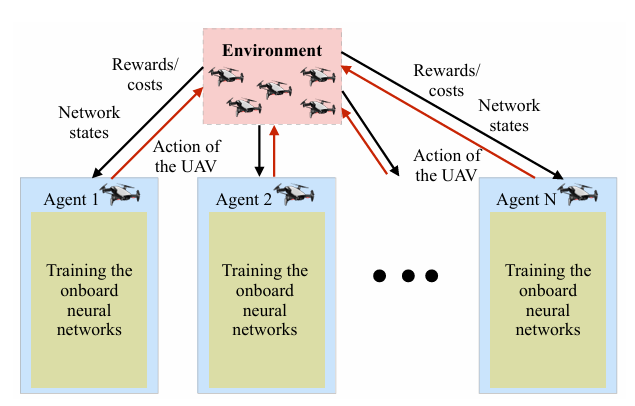
\includegraphics[width=0.8\textwidth]{Figures/Chapter2/Section1/5.png}
\caption{A multi-agent DRL structure where each UAV trains an onboard neural network to determine the optimal joint actions~\cite{kurunathan2022machine}}
\label{multi_agent_drl_structure}
\end{figure}

\textbf{Note:} The selection between multi-agent DQN and DDPG implementations depends on the action space characteristics of the target application. DQN is preferred for discrete decision spaces (e.g., UAV clustering), while DDPG excels in continuous control scenarios (e.g., precise trajectory planning). Complementary techniques like autoencoding further enhance these frameworks through efficient feature extraction and supervised learning components.







%%%%%%%%%%%%%%%%%%%%%%%%%%%%%%%%%%%%%%%%%%%%%%%%%%%%%%%%%%%%%%%%%%%%%%

\subsection{Machine Learning for UAV Perception and Feature Extraction}


Feature extraction is a technique for reducing dimensionality. It typically begins with a set of real-time data collected through the UAV's camera, followed by the creation of derived values (such as edges, shapes, and object recognition) that carry meaningful information. This derived learning is non-redundant and supports subsequent learning to enhance feature extraction. Unlike traditional imaging platforms, UAVs offer a unique vantage point, providing an expansive view of the area of interest. Additionally, the mobility of UAVs allows them to cover a larger geographical area compared to stationary imaging systems. In the following sections, we explore key machine learning techniques applied to UAV-assisted imaging.


\subsubsection{Supervised Learning-based UAV Operations}



Supervised machine learning techniques, like MLP, are capable of processing information through multiple layers, assisting in the interpretation of images captured by the UAV. Approaches such as CNN can segment and link the layers of an image, facilitating feature extraction.

\begin{enumerate}
    \item \textbf{Multilayer Perceptron for Image Processing}

    UAVs have gained significant traction in precision agriculture, particularly in crop disease analysis and vegetation management, where MLP models demonstrate notable effectiveness. In \cite{Abdulridha2020}, a UAV equipped with hyperspectral cameras captures hyperspectral images of a tomato field to facilitate early disease detection caused by fungus and bacteria. An MLP neural network classifies the images, achieving an impressive accuracy rate of 99\%. In an other approach a quadcopter UAV, outfitted with a Raspberry Pi single-board computer and an onboard camera module, is employed for vegetation mapping in tomato crops. MLP is used to segment the crop images, outperforming the support vector machine (SVM) alternative in terms of precision and recall.

    The utility of MLP in aerial image analysis extends beyond agriculture to environmental management, such as weed eradication \cite{Tamouridou2017}. In this study, a multi-spectral camera is mounted on an eBee fixed-wing UAV to capture high-resolution images of a field. An MLP with automatic relevance detection (MLP-ARD) is used to detect the weed species *Silybum marianum* among various types of vegetation. The MLP, featuring one hidden layer and one output unit, is regulated through Bayesian regularization to prevent overfitting and is trained on spectral and textural input data to classify the weed effectively. MLP has also been applied to flood management, with UAVs capturing aerial images of flooded areas in Houston, Texas. In this case, an MLP is used for semantic analysis following the use of a densely connected CNN and RNN to process the images.
    
    Furthermore, MLP models have proven useful in UAV route planning and agricultural harvesting. In \cite{annepu2020uav}, UAVs assist in route planning and harvest volume estimation for unmanned agricultural harvesting systems, addressing the challenge of harvest losses due to untimely collection. The UAV, equipped with multi-spectral cameras, captures images that are analyzed using various neural networks, including MLP. The MLP, with three neurons in the hidden layer, provides optimal performance compared to other tested models, such as generalized regression networks and radial basis function networks.
    

    
    \item \textbf{Convolutional Neural Network for Image Processing}

    CNN is widely utilized for classifying and segmenting remotely sensed imagery due to its ability to extract detailed features. In UAV forest imagery, CNN can effectively identify features such as vegetation and dry areas. It is also employed in multi-object tracking for real-time applications, where it associates objects efficiently. Challenges arise from poor radio connections between the UAV and the base, which can degrade the quality of transmitted images, leading to packet loss and bandwidth wastage. A solution for this issue involves an Optimal Strategy Library (OSL) for video encoding, which adapts to the packet loss rate and bandwidth, ensuring improved video sequence encoding and recovery of partially corrupted videos \cite{kurunathan2022machine}.
    
    CNN-based approaches have shown high precision and accuracy (around 90\%) in detecting slope failures from UAV remote sensing imagery. Similar performance is observed in several other image classification applications, where CNN achieves over 90\% accuracy. In high-throughput phenotyping using high-resolution multispectral imaging, CNN classification and segmentation techniques provide nearly 99\% accuracy. For search and rescue operations, UAVs with video cameras can analyze avalanche debris, and CNN can identify features indicative of survivors. Additionally, a linear Support Vector Machine (SVM) can be used in conjunction with CNN to enhance object detection.
    
    CNN excels in imaging applications such as localization, object detection, and segmentation. Despite its strengths, one limitation is the time, energy, and resources required for segmentation tasks. To address this, techniques like recurrent CNN (R-CNN) have been developed to streamline the processing. In certain UAV imagery applications, R-CNN improves detection accuracy and resolves issues related to image resolution. Lightweight CNN architectures have also been proposed for efficient execution on embedded processors, providing a balance between performance and resource consumption. Energy-aware designs have been suggested to minimize power consumption in UAV tracking and landing tasks, with CNN's Quality of Service (QoS) level adjusting to save energy.
    
    Although CNN is highly effective, it does not encode object position and orientation, and its detailed segmentation process can be resource-intensive. The layers closer to the CNN input focus on simple features such as edges, corners, and endpoints, but deeper layers, which offer more complex feature extraction, require longer training times. To mitigate this, lightweight CNN models have been introduced to reduce the need for powerful GPUs. Additionally, integrating Recurrent Neural Networks (RNN) with CNNs has shown promise in improving image processing, where dense connections enhance information flow and gradient propagation, thus improving training efficiency and reducing overfitting. This integration has achieved impressive results, with reported accuracy rates of 96\% on real-world datasets.
    

    \begin{figure}[H]
        \centering
        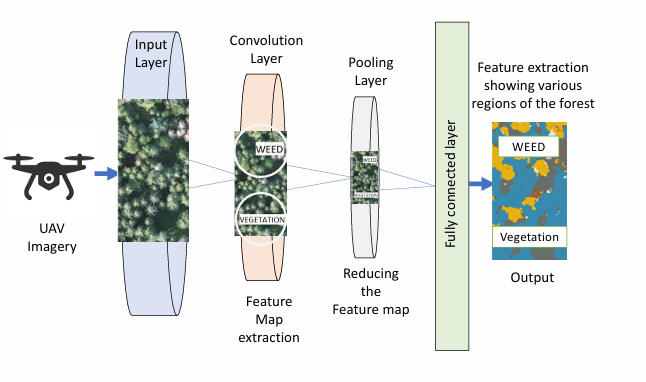
\includegraphics[width=0.7\textwidth]{Figures/Chapter2/Section1/6.png}
        \caption{Convolutional Neural Networks in Image Processing~\cite{kurunathan2022machine}}
        \label{cnn_image_processing}
    \end{figure}

\end{enumerate}



\subsubsection{Unsupervised Learning-based Approaches}
    
    Novel unsupervised learning techniques, such as spiking neural networks (SNN), have energy-efficient and high-processing capabilities, making them suitable for faster and more energy-efficient control decisions in UAV operations. Neuromorphic SNNs utilize temporal difference learning to predict both rewards and temporal sequences in physical time. Temporal difference learning can be achieved by analyzing the temporal distance between neighboring events that vary in decay time constant. Neuromorphic SNNs replicate the functionality of a central nervous system, and typically operate at orders of magnitude lower power than traditional computing systems. This low-power capability is due to the event-driven, massively parallel nature of SNNs, where only a small portion of the system is active at any given time while the rest remains idle. This makes them suitable for applications such as edge computing, where strict energy constraints exist \cite{kurunathan2022machine}. 


    \begin{figure}[H]
        \centering
        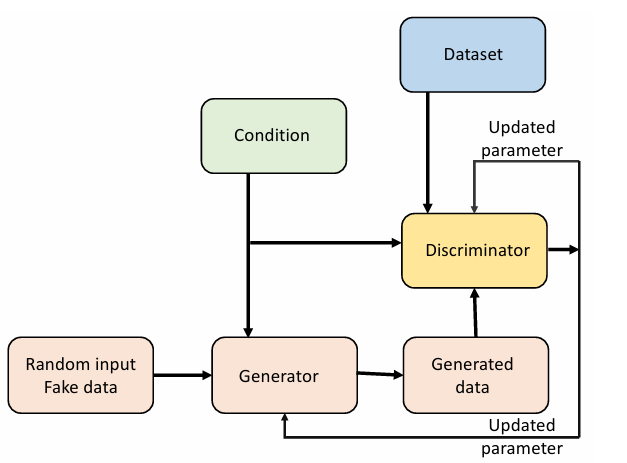
\includegraphics[width=0.7\textwidth]{Figures/Chapter2/Section1/7.png}
        \caption{Generative Adversarial Network Framework for UAVs~\cite{kurunathan2022machine}}
        \label{GAN_UAV}
    \end{figure}
    To leverage the ultra-low-power capabilities of neuromorphic processors (on the order of several milliwatts), a neuromorphic SNN model has been studied for onboard deployment in UAVs to control their movements for obstacle avoidance. Differential evolution and Bayesian optimization are used to obtain the optimal configuration for the SNN. An SNN-based proportional-integral-derivative (PID) controller has been integrated with UAV motor control to ensure ultra-low power consumption while maintaining a high processing rate. In this architecture, each spiking neuron carries sensor measurements and control information, firing a spike when thresholds or biases are reached.
    
    SNNs are also studied to control a hexacopter UAV in six degrees of freedom: yaw, roll, pitch, height, position, and angular velocity. A recurrent spiking controller is proposed to solve nonlinear control problems in continuous domains using a topology evolution algorithm as the learning mechanism. The results suggest that SNNs can solve ongoing control problems by maintaining sufficient spike activities and decoding from weighted spike frequencies. Additionally, an unsupervised Spike Time Dependent Plasticity (STDP) approach has been developed to detect UAVs in images. This asynchronous system, utilizing event-based camera features, is both low in power consumption and computational overhead.
    
    A decision-making model for UAV flight control uses an SNN to simulate brain zone functions, determining control actions based on the relative positions of obstacles and the UAV. A system has been developed where spiking neurons detect and locate obstacles by partitioning the onboard camera image and mapping it for navigation. One SNN model, the liquid state machine, can track network states over time and predict data feature distributions. Liquid state machines have also been applied to resource allocation in cache-enabled UAVs, learning the data request distribution from ground nodes and determining data caching policies for the UAV.
    
    % \textbf{Remark:} Due to their ability to process data recurrently and constantly learn from the environment, methods like RNNs are well-suited for UAV control. Techniques like SNNs bring the advantage of energy efficiency to UAV operations. Machine learning (ML) methods are also used for real-time waypoint setting and smart trajectory planning for applications such as data collection and sensing.
    
    
%%%%%%%%%%%%%%%%%%%%%%%%%%%%%%%%%%%%%%%%%%%%%%%%%%%%%%%%%%%%%%%%%%%%%%

\subsection{Machine Learning for Feature Interpretation and Regeneration}


Feature extraction is a form of dimensionality reduction. Feature extraction, pattern recognition, and image processing usually start from an actual set of measured data (taken through the camera of the UAV). It builds derived values (features such as edges, shapes, object recognition) that are informative. This derived learning is non-redundant and facilitates subsequent learning to obtain better feature extraction. UAVs can provide an eagle-eyed view of the region of interest compared to their counterparts, i.e., the non-UAV imaging platforms. The mobility of UAVs can also provide the capability to cover a larger geographical area than their stationary counterparts \cite{244}. In what follows, we discuss important ML techniques used in UAV-assisted imaging.


\subsubsection{Feature interpretation by Linear Regression}



The use of UAVs for environmental observation and agricultural monitoring has been growing steadily. These aerial platforms collect various types of sensory data through onboard instruments like cameras and infrared sensors. One of the most widely adopted techniques for analyzing such data is linear regression (LR), along with its different extensions.

Linear regression, a core technique in supervised machine learning, is employed to model the relationship between a set of input features and a continuous target output. This approach provides numerical insight into how features influence the target variable, offering a way to explain and quantify feature importance.

In one application, LR was used to evaluate how the spatial placement of sensors affects air pollution measurements in a UAV-based system \cite{villa2016uav}. This study also proposed design guidelines for UAV systems tasked with locating emission sources.

In the field of precision agriculture, LR helped establish a correlation between the crop coefficient and the normalized difference vegetation index to estimate evapotranspiration \cite{niu2020estimating}. A deep stochastic configuration network was also utilized to complement the LR model and enhance predictive performance.

Other research combined plant height and vegetation indices derived from UAV imagery to estimate biomass using a multiple LR model. Additionally, structure-from-motion (SfM) techniques were applied to generate 3D point clouds from overlapping aerial images. These were used to evaluate the health of wetland vegetation by linking them to vegetation indices through LR models.

In bathymetric mapping, LR’s limitations were addressed by introducing a geographically weighted regression (GWR) model, which improved accuracy and reduced the spatial biases often present in standard multiple regression approaches .

For soil salinity mapping, advanced regression techniques such as random forest models were applied on data collected from electromagnetic induction sensors and hyperspectral cameras.

Although LR is easy to implement and interpret, it assumes a linear relationship between inputs and outputs. This assumption can lead to poor model performance when the actual relationship is more complex. Furthermore, LR is sensitive to noise and prone to overfitting, especially when the number of input features exceeds the number of available observations.



\subsubsection{Classification by K-Means Clustering}

K-means clustering has been effectively applied in path planning for multi-UAV systems, particularly when coordinating multiple tasks within a designated area. Given the geographic distribution of tasks, K-means is used to group them into several clusters. Each cluster can then be assigned to a UAV, and route optimization techniques such as simulated annealing or genetic algorithms are employed to determine efficient paths within those clusters.

In addition to task allocation, K-means plays a role in guiding UAV movement for coverage-related objectives. For instance, in scenarios where UAVs are deployed to deliver cellular connectivity, the approach dynamically groups users based on their spatial positions. UAVs are then directed to the centroids of these groups to ensure adequate coverage and maintain service quality. This method has demonstrated convergence toward locally optimal deployments. Similar strategies have also been implemented in aerial surveillance tasks to ensure efficient area monitoring using multiple UAVs.







    \begin{figure}[H]
        \centering
        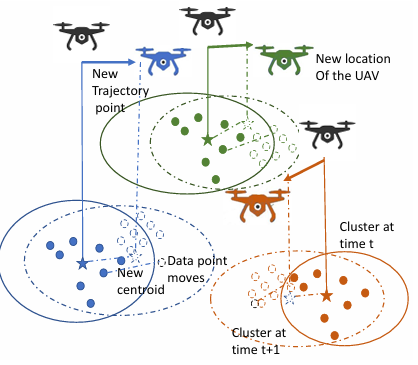
\includegraphics[width=0.7\textwidth]{Figures/Chapter2/Section1/8.png}
        \caption{Centroid-Based Coordination in Multi-UAV Surveillance Using K-Means Clustering~\cite{huang2021navigating}}
        \label{centroid_kmeans_uav}
    \end{figure}








\subsubsection{Environment Modeling Using Gaussian Mixture Models}


GMM (Gaussian Mixture Model) is applied to model static, complex-shaped, two-dimensional obstacles, aiding in the prevention of UAV collisions. Given prior probabilistic knowledge about obstacles, GMM is generated to form the potential field of the target area. The parameters of the GMM are iteratively estimated using the Expectation-Maximization (EM) method, allowing the model to approach the true distribution of the obstacles. By taking derivatives over the GMM, the potential field is created, and UAV flight paths are determined by following the field directions. A trajectory prediction model based on GMM clusters trajectory data into distinct components and applies Gaussian process regression to predict possible future trajectories. Additionally, GMM is utilized to create heatmaps of object detection probabilities in a designated area. For instance, a UAV can be used to maximize the probability of locating a specific object by planning an efficient flight path, taking into account environmental factors like foliage coverage, shadowing, and illumination. The spatial distribution of detection probabilities is modeled using GMM, which aids in creating a hierarchical search plan for a mission. 


    \begin{figure}[H]
        \centering
        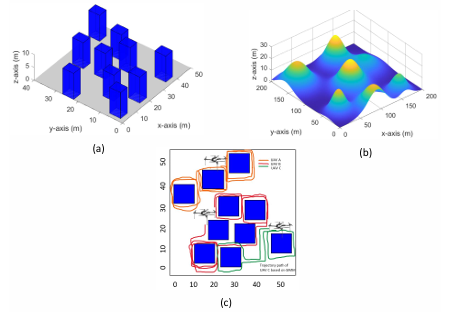
\includegraphics[width=0.7\textwidth]{Figures/Chapter2/Section1/9.png}
        \caption{Trajectory Planning for UAVs Using GMM-Based Environment Modeling~\cite{huang2021navigating}}
        \label{trajectory-planning-gmm}
    \end{figure}





Furthermore, GMM is integrated with horizon control techniques to optimize the trajectories of multiple UAVs tasked with searching a complex environment. In these setups, receding horizon control (model predictive control, MPC) is used for dynamic path planning to optimize search efforts, avoid collisions, and ensure simultaneous arrival at a target. Cooperation among UAVs is facilitated by regular flight path broadcast messages. GMM is also used to model the distribution of radio traffic in cellular networks involving UAV-based base stations (BSs), which helps in optimizing UAV placement. By utilizing a weighted EM algorithm, GMM can predict traffic congestion and reduce UAVs' energy consumption for communication and mobility. Simulations indicate a reduction of 20\% in communication energy use and 80\% in mobility energy compared to heuristic methods.

In conclusion, techniques such as K-means clustering and linear regression are effective in feature interpretation and environmental data analysis, while probabilistic models like GMM excel at spatial distribution modeling and feature classification. These methods prove highly accurate when sufficient prior data is available, enabling complex applications like UAV control.




%%%%%%%%%%%%%%%%%%%%%%%%%%%%%%%%%%%%%%%%%%%%%%%%%%%%%%%%%%%%%%%%%%%%%%
%%%%%%%%%%%%%%%%%%%%%%%%%%%%%%%%%%%%%%%%%%%%%%%%%%%%%%%%%%%%%%%%%%%%%%
%%%%%%%%%%%%%%%%%%%%%%%%%%%%%%%%%%%%%%%%%%%%%%%%%%%%%%%%%%%%%%%%%%%%%%









% \section{Security in UAVs networks}


% \subsection{taxonomy of security threats based on threat vectors}

%     This section introduces a structured overview of security threats in FANETs, organized according to threat vectors, as depicted in Figure~\ref{fig:FANET_threats}. These vectors include six types of connections and six distinct node categories. A total of 20 threats are analyzed and categorized based on both their impact on security requirements and their relevance to different network architectures.
    
%     Utilizing the STRIDE threat modeling framework, we identify specific vulnerabilities affecting both node and connection layers (see Figure~\ref{fig:FANET_threats}). 
    
%     Out of the 20 threats, 15 pertain to connection-level vulnerabilities, while the remaining five are associated with node-level issues. To address these threats, 15 mitigation strategies have been proposed. These strategies span six types of networks: 5G mobile networks, FANETs, general Ad-Hoc networks, RW, WLAN, and WSN.
    
    


%     \begin{figure}[H]
%         \centering
%         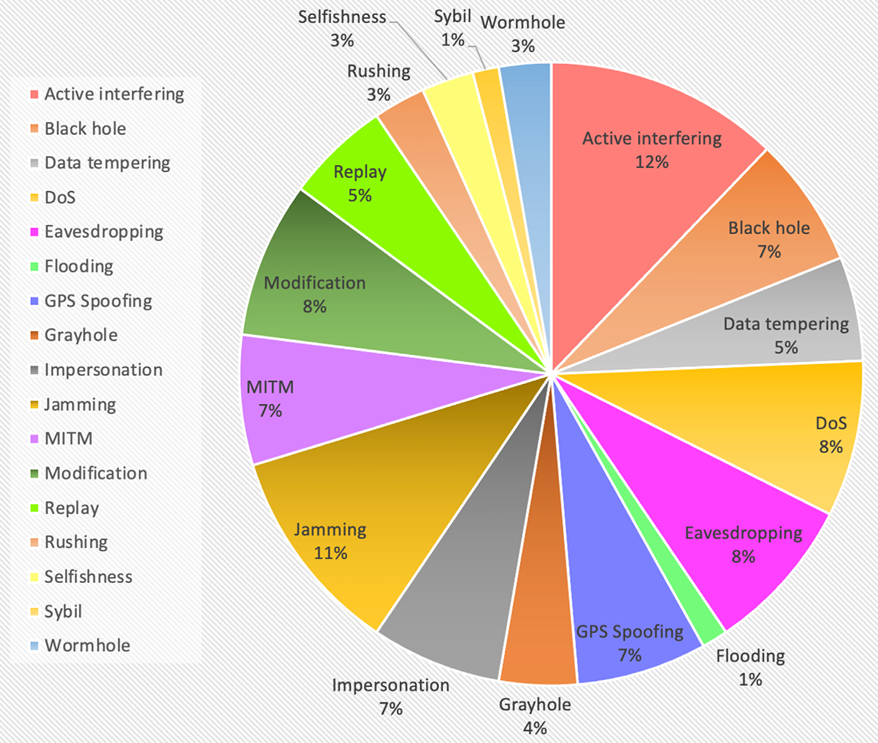
\includegraphics[width=0.7\textwidth]{Figures/Chapter2/Section2/1.png}
%         \caption{Percentage of security threats in FANETs~\cite{tsao2022survey}}
%         \label{fig:FANET_threats}
%     \end{figure}
    

% \subsubsection{Threat vectors}








% The following section analyzes the primary security threats that can affect each communication link within a typical UAV ground and aerial system. These links ranging from user interfaces to inter-UAV communication are potential vectors for attacks targeting confidentiality, integrity, availability, or authenticity. For each connection, we identify common threats and describe them succinctly for clarity and reference.

% \paragraph{C1: Client terminal to GCS.}

% This connection involves the user interface where operators input commands or receive feedback. It is vulnerable to insider misuse, eavesdropping, and message replay.

% \begin{itemize}
%     \item \textbf{Eavesdropping:} Interception of sensitive data such as commands or credentials, which compromises confidentiality.
%     \item \textbf{Insider threat:} Authorized users misusing their access to compromise the system's integrity.
%     \item \textbf{Replay attack:} Reuse of captured messages to produce misleading outcomes, affecting authenticity.
% \end{itemize}

% \paragraph{C2: GCS to Backbone UAV.}

% This link is critical for command and control and is transmitted via wireless media that differ in vulnerability. The security depends heavily on the medium used.

% \begin{table}[H]
% \renewcommand{\arraystretch}{1.3}
% \centering
% \caption{Transmission medium vulnerabilities for C2.}
% \begin{tabular}{|>{\centering\arraybackslash}m{3.5cm}|
%                 >{\centering\arraybackslash}m{2.5cm}|
%                 >{\arraybackslash}m{7.5cm}|}
% \hline
% \textbf{Medium} & \textbf{Security Level} & \textbf{Vulnerabilities} \\
% \hline
% WiFi & Medium & Susceptible to interception if not strongly encrypted; can be mitigated using non-standard frequency bands. \\
% \hline
% RF & Low & Sensitive to interference; careful channel selection and control are needed. \\
% \hline
% Satellite & High & Generally more secure but expensive and less commonly used in civilian operations. \\
% \hline
% \end{tabular}
% \label{tab:c2_mediums}
% \end{table}

% \vspace{1em}

% The communication from GCS to UAVs is open to several attacks, particularly due to wireless exposure. The table below details key threats targeting this path.

% \begin{table}[H]
% \renewcommand{\arraystretch}{1.3}
% \centering
% \caption{Threats on the GCS–Backbone UAV connection (C2).}
% \begin{tabular}{|>{\centering\arraybackslash}m{3.5cm}|
%                 >{\centering\arraybackslash}m{2.5cm}|
%                 >{\arraybackslash}m{7.5cm}|}
% \hline
% \textbf{Threat} & \textbf{Category} & \textbf{Description} \\
% \hline
% Eavesdropping & Confidentiality & Leakage of mission-critical information or positioning data. \\
% \hline
% Jamming & Availability & Intentional or accidental signal disruption, breaking communication. \\
% \hline
% Man-in-the-middle & Integrity & Interception and manipulation of exchanged messages. \\
% \hline
% Replay attack & Authenticity & Reusing valid packets to disrupt or trick the communication logic. \\
% \hline
% \end{tabular}
% \label{tab:c2_threats}
% \end{table}

% \paragraph{C3 and C4: Backbone UAV to other UAVs.}

% These connections support swarm behavior and inter-UAV coordination. Their wireless nature makes them highly sensitive to disruptions and impersonation threats.

% \begin{table}[H]
% \renewcommand{\arraystretch}{1.3}
% \centering
% \caption{Threats on Backbone-to-UAV and inter-UAV connections (C3, C4).}
% \begin{tabular}{|>{\centering\arraybackslash}m{3.5cm}|
%                 >{\centering\arraybackslash}m{2.5cm}|
%                 >{\arraybackslash}m{7.5cm}|}
% \hline
% \textbf{Threat} & \textbf{Category} & \textbf{Description} \\
% \hline
% Eavesdropping & Confidentiality & Unauthorized interception of UAV status or swarm coordination commands. \\
% \hline
% Jamming & Availability & Signal blocking that affects the swarm’s ability to coordinate. \\
% \hline
% Man-in-the-middle & Integrity & Rogue UAVs impersonate legitimate ones to alter, delay, or block communication. \\
% \hline
% Replay attack & Authenticity & Repetition of past messages to cause confusion or misalignment in swarm behavior. \\
% \hline
% \end{tabular}
% \label{tab:c3_c4_threats}
% \end{table}






% \subsubsection{Security threats on nodes}

% Security threats on nodes, including client terminals, GCS, and UAVs, can disrupt FANET operations. If a node fails to forward messages, another node may take control of the mission.

% \textbf{Client terminal.} Client terminals can be attacked to send malicious or fake commands, depending on their hardware and operating systems.

% \textbf{GCS and backbone UAV, single point of failure (SPOF).} The reliance on a single GCS and backbone UAV is a vulnerability. Implementing multiple GCSs and UAVs enhances resilience by ensuring automatic operation in case of failure.

% \textbf{UAVs.} UAVs face several major threats:

% \begin{itemize}
%     \item \textbf{Backdoor.} UAVs can contain backdoors that allow external control, hijacking their operation. ~\ref{fig:Maldrone_Attack} shows a Maldrone attack.

%     \begin{figure}[H]
%         \centering
%         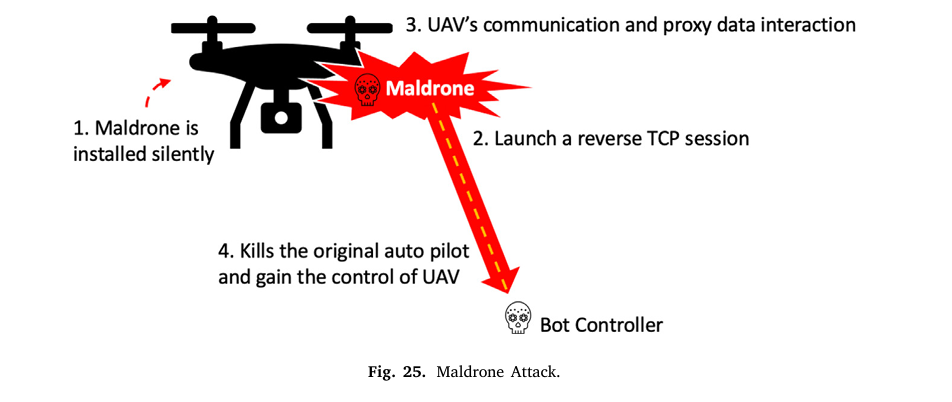
\includegraphics[width=0.7\textwidth]{Figures/Chapter2/Section2/4.png}
%         \caption{ Maldrone Attack ~\cite{tsao2022survey}}
%         \label{fig:Maldrone_Attack}
%     \end{figure}
    
%     \item \textbf{Denial of Service (DoS) attack.} Attackers can overload UAVs with fake messages, preventing new missions or disrupting flight paths. ~\ref{fig:DoS_Attack} shows a DoS attack on UAV 1.

%     \begin{figure}[H]
%         \centering
%         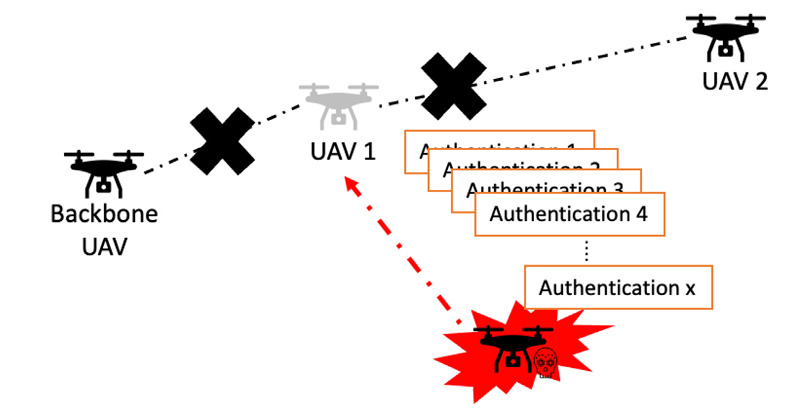
\includegraphics[width=0.7\textwidth]{Figures/Chapter2/Section2/5.png}
%         \caption{  DoS Attack ~\cite{tsao2022survey}}
%         \label{fig: DoS_Attack}
%     \end{figure}
    
%     \item \textbf{Flooding attack.} Sending large volumes of data to UAVs can deplete their resources, causing malfunctions.
    
%     \item \textbf{Selfishness/selfish node.} UAVs low on energy may reduce performance by failing to forward data to others, degrading network efficiency. ~\ref{fig:IOD_system} shows an example of a selfish node

%     \begin{figure}[H]
%         \centering
%         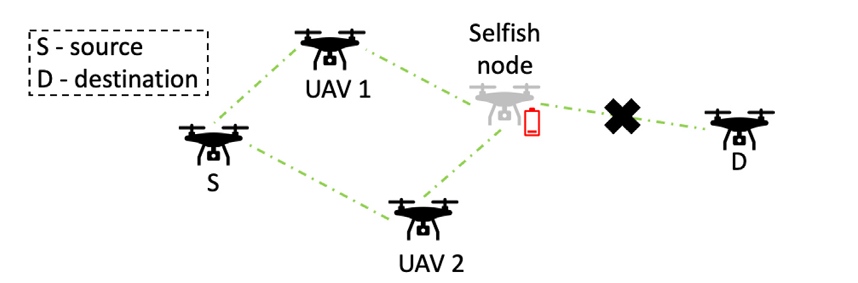
\includegraphics[width=0.7\textwidth]{Figures/Chapter2/Section2/6.png}
%         \caption{  Selfish Node ~\cite{tsao2022survey}}
%         \label{fig: Selfish_Node}
%     \end{figure}
    
%     \item \textbf{Cloud server and storage, data tampering.} Modifying stored data in cloud databases can compromise privacy or disrupt operations.
% \end{itemize}



% \subsubsection{Security threats on the IoD}

% The Internet of Drones (IoD) faces several security and privacy challenges. Drones often lack built-in protections, making them prone to data leaks and attacks. Hardware constraints lead to reliance on lightweight encryption and processing protocols. Airspace is divided into zones connected by gates, with each zone having mapped routes and intersections. Zone Service Providers (ZSPs) deliver navigational data to assist drone operations. Figure~\ref{fig:IOD_system} illustrates the overall structure of the IoD communication system.


% \subsubsection{Confidentiality}
% IoD systems handle sensitive data such as locations, flight paths, and drone identities, which could be exploited for physical attacks. Systems must support drone identification when needed, while minimizing exposure. Insider threats, including personnel with privileged access, can pose significant risks.

% \subsubsection{Integrity}
% Limited processing power in drones and ZSPs leads to offloading tasks to cloud services. Unencrypted data is vulnerable to unauthorized access. Large datasets like video streams may be difficult to encrypt, and even when encrypted, processing limitations hinder efficient indexing and search.

% \subsubsection{Availability}
% ZSP-drones communication links are attractive targets for denial-of-service, spoofing, and data injection attacks. These threats may require external auditing to detect. Trusted computing platforms can help enforce system integrity, though they may introduce latency or false alarms.

%     \begin{figure}[H]
%         \centering
%         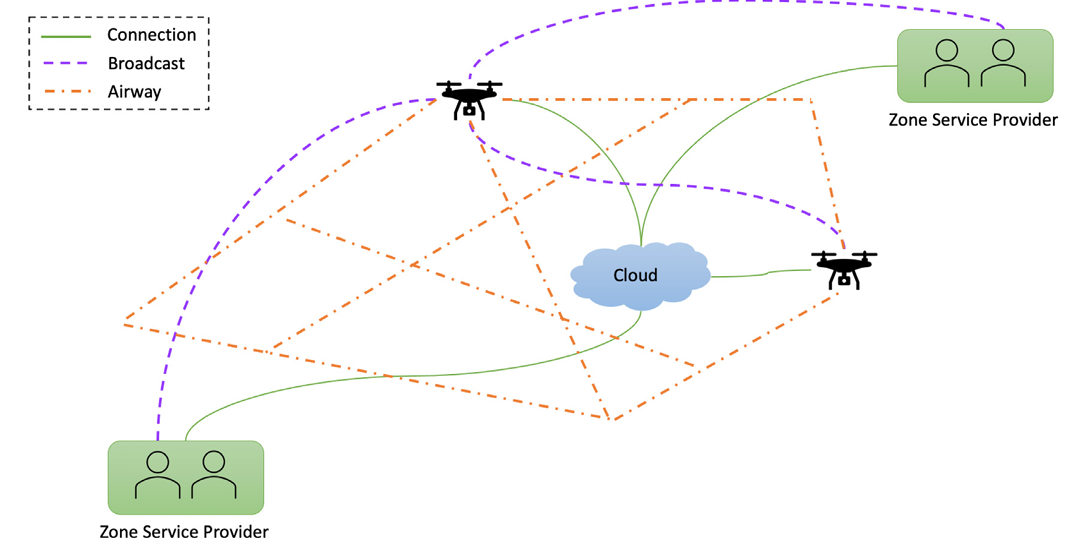
\includegraphics[width=0.7\textwidth]{Figures/Chapter2/Section2/3.png}
%         \caption{ IoD Communication System Overview ~\cite{tsao2022survey}}
%         \label{fig:IOD_system}
%     \end{figure}

% %%%%%%%%%%%%%%%%%%%%%%%%%%%%%%%%%%%%%%%%%%%%%%%%%%%%%%%%%%%%%%%%%%%%%%
% \section{Security solutions and standards}

% As UAVs in Flying Ad-Hoc Networks (FANETs) become more prevalent, securing their communication and operations against various threats is essential. These threats include jamming, malware, data tampering, and blackhole attacks, among others. This section examines the key security challenges in FANETs and outlines the solutions developed to address them. These solutions vary from agent-based approaches, which rely on UAV-specific agents, to agent-less methods, depending on the resources available. The section also covers essential security requirements, such as availability, confidentiality, and integrity, which are critical to ensuring the secure operation of UAV networks.

%     \begin{figure}[ht]
%         \centering
%         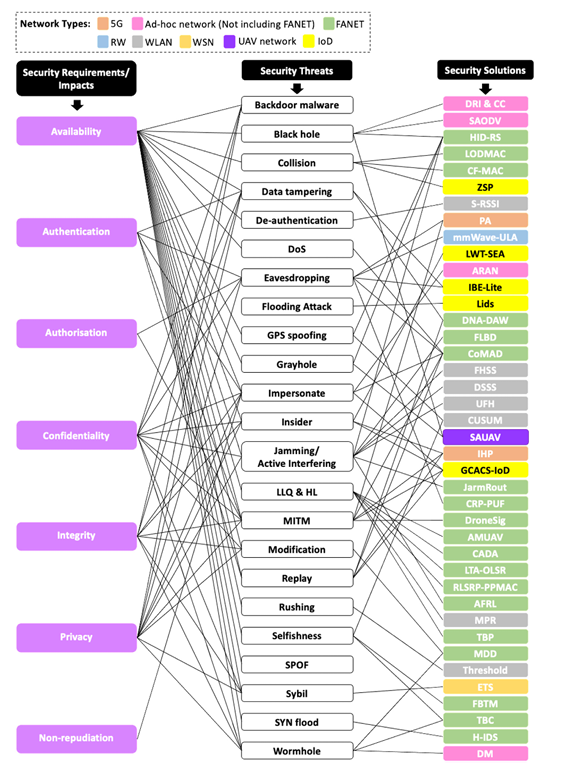
\includegraphics[width=0.7\textwidth]{Figures/Chapter2/Section2/7.png}
%         \caption{ Security threats and solutions based on security requirements ~\cite{tsao2022survey}}
%         \label{fig:threats_solutions}
%     \end{figure}

% \subsubsection{Active interfering (jamming)}

% Multiple solutions have been developed to address various security threats in FANETs. These include protections against denial of service (DoS), eavesdropping, impersonation, man-in-the-middle (MITM), replay, blackhole and grayhole attacks, GPS spoofing, jamming, collisions, data tampering, and insider threats.

% Security methods are generally classified as agent-based or agent-less. Agent-based solutions use device agents, often enhanced by autonomous machine learning algorithms, while agent-less solutions operate without background services. The choice depends on the UAVs’ computational power and application needs.

% A security framework outlines twenty-three threats and seven main requirements: availability, confidentiality, privacy, integrity, authentication, authorization, and non-repudiation. Availability stands out as the most critical in FANET environments.

% \subsubsection{Backdoormalware}

% Currently, there is no specific solution addressing UAV backdoor malware that ensures the confidentiality, availability, integrity, and privacy of FANET communications. While some methods have been developed for mobile nodes in wireless sensor networks, they are not specifically designed for FANET or UAV environments. However, certain techniques involving the detection, tracking, and neutralization of infected nodes may offer potential for addressing future security challenges in UAV networks.


% \subsubsection{Blackhole}

% The Ad-hoc On-demand Distance Vector (AODV) protocol is vulnerable to blackhole attacks, which can disrupt network integrity. Several solutions have been proposed to enhance FANET availability and prevent packet loss by malicious nodes \cite{sen2011mechanism}.

% One solution \cite{sen2011mechanism} uses a secure agent unmanned aerial vehicle (SAUAV) system based on AODV. It operates in two phases: first, identifying and removing malicious UAVs, and second, enabling UAVs to discover neighbors and share information about malicious nodes. This method effectively detects malicious nodes and ensures high packet delivery rates with minimal false positives.

% % Another modification to AODV introduces Data Routing Information (DRI) tables and Cross Checking (CC). Each node tracks packet routes through its own DRI. During route discovery, the source node broadcasts a Route Request (RREQ), and an intermediate node responds with a Route Reply (RREP), allowing the source to verify the route's reliability. This helps mitigate blackhole attacks by ensuring only trusted routes are used.

% A Secure AODV (SAODV) protocol targets blackhole attacks by ignoring the first reply packet from the source node, assuming malicious nodes reply first. This approach filters out malicious nodes attempting to hijack the route discovery process.

% Additionally, a hierarchical detection and response system (HID-RS) uses a centralized Ground Control Station (GCS) to monitor FANET packets. UAVs send neighboring packets to the GCS, which classifies them as normal, suspect, abnormal, or malicious. The GCS then verifies if relay UAVs send packets and calculates dropped packets. A threshold is set and updated with a Support Vector Machine (SVM) to differentiate between intentional and unintentional packet drops.


% \subsubsection{Collisions}

% UAVs can operate in, join, or leave half-duplex FANET networks, which are characterised by high mobility levels and frequent topology changes. Therefore, the MAC layer must provide collision-free communication and enhance the availability of the FANET. The location-oriented directional MAC protocol (LODMAC) increases FANET capacity and availability by integrating neighbouring UAV locations with directional antennas, resolving issues such as collisions and deafness. A collision-free MAC protocol (CF-MAC) uses the CSMA/TDMA MAC protocol with a half-duplex radio channel and omni-directional antennas. To prevent collisions, time slots are assigned to regulate how UAVs join the network. Additionally, to maintain effective and real-time navigation, only authorised UAVs should operate in specific aerial spaces. UAVs broadcast their location to a zone service provider (ZSP), which detects, monitors, and manages UAV operations, checking for abnormal behaviour, such as denial of service (DoS), spoofing, or data tampering attacks that could disrupt normal network operation.









%%%%%%%%%%%%%%%%%%%%%%%%%%%%%%%%%%%%%%%%%%%%%%%%%%%%%%%%%%%%%%%%%%%%%%

\section{Conclusion}

AI and optimization techniques have revolutionized UAV applications, enabling smarter path planning, resource management, and autonomous decision-making. Reinforcement learning methods like DQN and DDPG have proven particularly effective in handling both discrete and continuous control tasks. However, as UAV networks expand, security threats such as data tampering and denial-of-service attacks demand stronger defenses, including protocols like SAODV and collision-free MAC layers. Future research should focus on lightweight AI models for real-time processing and resilient encryption methods to safeguard UAV communications. This chapter highlights the synergy between AI advancements and security measures, emphasizing both the progress made and the challenges that remain in UAV technology.